\section{Theory: Neural dynamics}
\label{sec:Neuron}
\begin{itemize}
\item Multicompartmental modeling
\item Cable equation
\item No current monopoles - trick needed for point neurons
\end{itemize}

Modelling of neurons is at the core of computational neuroscience, and the topic has been treated in detail in several text books (see e.g., \cite{johnston1994foundations, KockSegev1998, Koch1999, Hille2001, Dayan2005, Sterratt2011}). We therefore only give a brief introduction to it here. 

Most simulations of extracellular potentials are based on biophysical multicompartmental neuronal models based on a formalism similar to that used in the celebrated model by Hodgkin and Huxley for membrane mechanisms (see e.g., \cite{Hodgkin1952, KockSegev1998, Pospischil2008}), and cable theory for how signals propagate in dendrites and axons (see, e.g., \cite{koch1999, rall2011}). We shall limit ourselves to present this framework, and we will refer to as the Hodgkin-Huxley-Cable (HHC) type framework. When we refer specifically to membrane mechanisms, we will refer to them as Hodgkin-Huxley (HH) type.

In the HHC-type framework, a neuron is characterized by (i) its morphology, and (ii) its membrane mechanisms. In a multicompartmental HHC-type model\index{multicompartment modelling}, the morphology of the real neuron (Fig. \ref{Neuron:fig:multicomp}A) is represented as a discretized set of compartments connected by resistors (Fig. \ref{Neuron:fig:multicomp}B). In such a model there are two categories of currents which together determine the membrane potential dynamics of the neuron (Fig. \ref{Neuron:fig:multicomp}C). These are the currents that run intracellularly between compartments (yellow arrows), and the transmembrane currents (green arrows). Once all the currents are characterized, the dynamics of the membrane potential can be computed by demanding that the sum of currents into a given compartment is zero (Kircchoff's current law). 

\begin{figure}[!ht]
\begin{center}
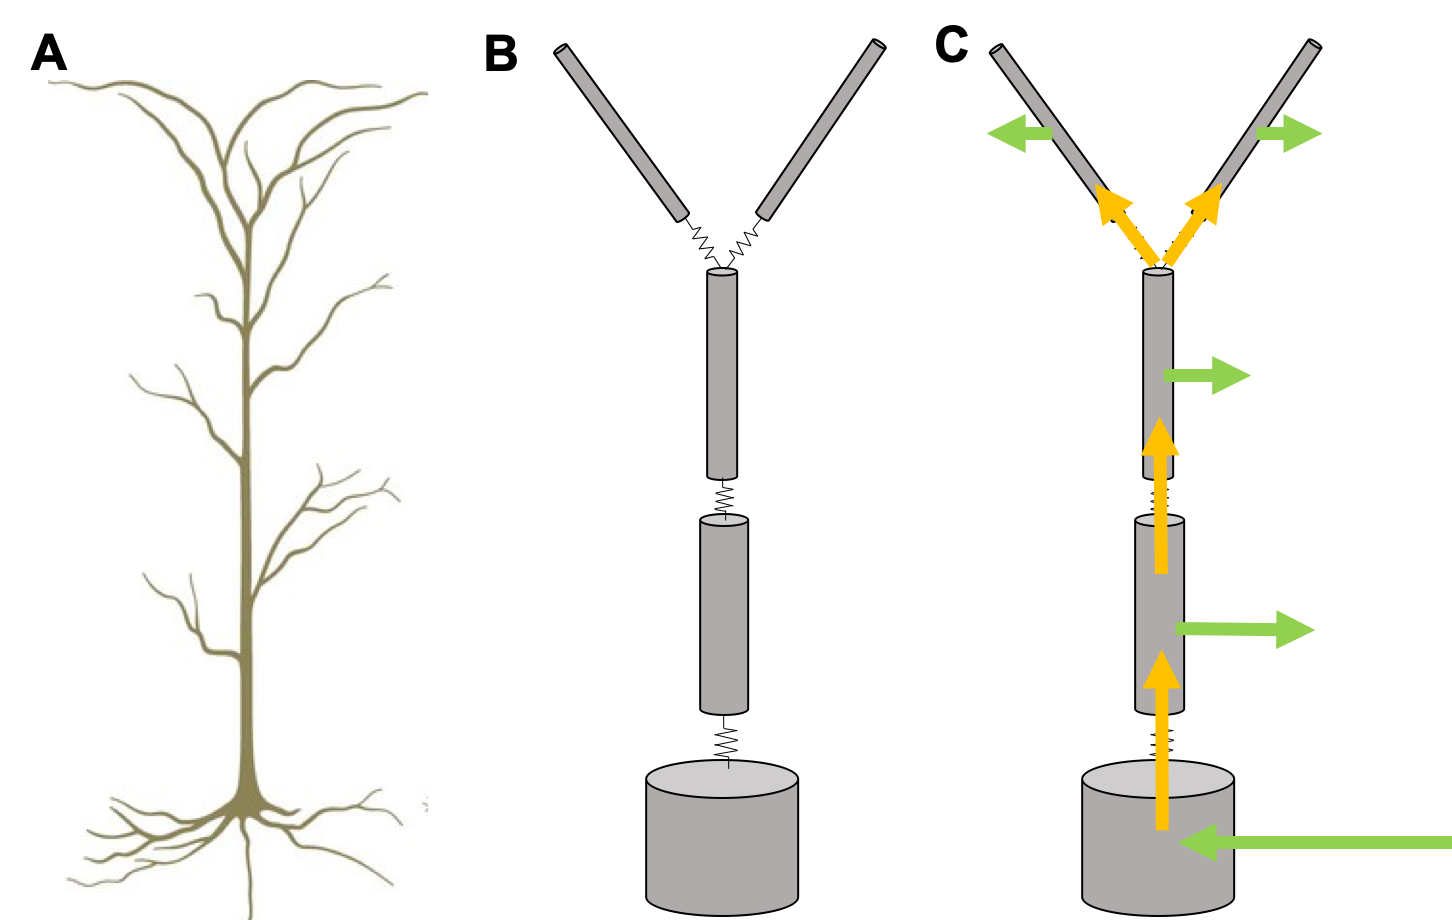
\includegraphics[width=0.6\textwidth]{Figures/Neuron/Multicomp.png}
\end{center}
\caption{\textbf{Multicompartmental modelling.} 
}
\label{Neuron:fig:multicomp}
\end{figure}

Below, we first present a framework for modeling the transmembrane currents in a single compartment (subchapter called "Membrane currents"), and next show how a number of such compartments can be connected together to a multicompartment model (subchapter called "Morphology").


\subsection{\blue{Membrane currents}}
In HHC-type models, the membrane typically includes three autonomous classes of transmembrane currents, normally represented as current densities (unit mA/cm$^2$). These are (i) a capacitive current density ($i_c$), (ii) a the leakage current density ($i_L$), and (iii) a the current density through active ion channels ($i_x$), of which there may be several different kinds ($x$ is an index). In addition, a neuron may receive  (iv) external stimuli ($i_{stim}$) either through synaptic currents or experimental current injections. In the case where the neuron is modeled as a single compartment, the net transmembrane current must be zero, so that:

\begin{equation}
i_c + i_L + \sum_x{i_x} +  i_{stim} = 0.
\label{eq:singlecomp_zerosum}
\end{equation}
Below, we define the various currents that go into this equation.

\subsubsection{\blue{Capacitive current}}
The capacitive current density,
\begin{equation}
i_c = c_m \frac{d\phi_m}{dt},
\label{eq:HHcap}
\end{equation}
represents the charging up of the membrane potential $\phi_m$ due to a charge density accumulating on the outside of inside of the capacitive membrane. Here, $c_m$ is the specific membrane capacitance. In the HH-model, $c_m$ had the value
1 $\mu$F/cm$^2$, and this value seems to be representative for most neurons.  An illustration of how to interpret the capacitive current is given in Fig. \ref{Neuron:fig:capacitive_currents}. 

\begin{figure}[!ht]
\begin{center}
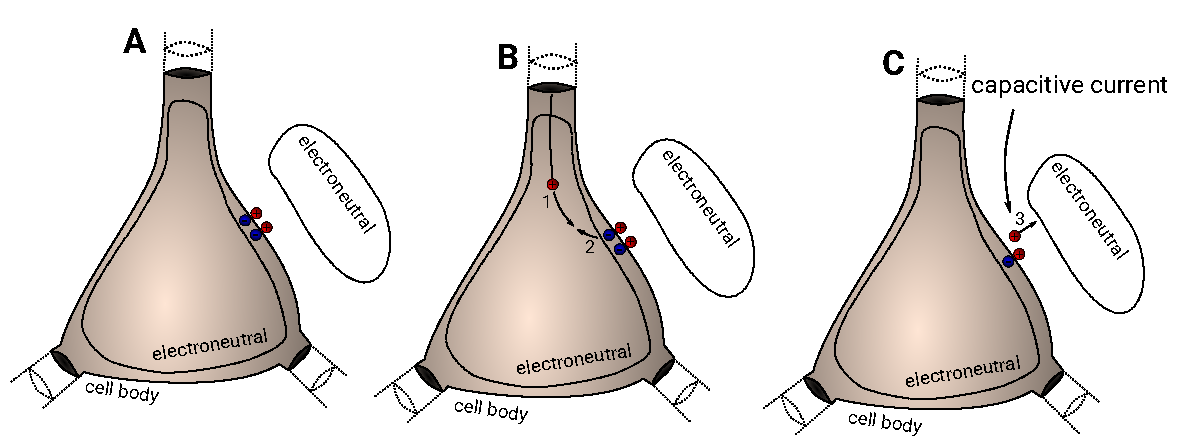
\includegraphics[width=0.8\textwidth]{Figures/Neuron/capacitive_currents.pdf}
\end{center}
\caption{\textbf{Capacitive currents are important for current conservation.}  (\textbf{(A)}) The extracellular and intracellular bulk solutions are essentially electroneutral, and the only region where there is a nonzero charge density is in thin Debye layers around the capacitive membrane. The capacitive current is not due to ions crossing the membrane, but due to ions piling up on either side of it, separating a charge density $\rho$ and a charge density $-\rho$, giving rise to a membrane potential of $\phi_m = \rho/c_m$. An outward capacitive current could correspond to an anion leaving the membrane on the inside (\textbf{(B)}), which will coincide with a cation leaving the membrane on the outside (\textbf{(C)}). Thus, capacitive membrane currents do give rise to electrical ionic volume currents both in the intra- and extracellular space.
}
\label{Neuron:fig:capacitive_currents}
\end{figure}


\subsubsection{\blue{Leakage current}}
The leakage current density is given by
\begin{equation}
i_L = \bar{g}_L (\phi_m - E_L),
\label{eq:HHleak}
\end{equation}
where $\bar{g}_L$ (mS/cm$^2$) is the leak conductance (the bar indicates that it's a constant). The factor $(\phi_m - E_L)$ (mV) is often called the driving force, and $E_L$ the leak reversal potential. The biophysical origin of the reversal potential is explained later (see SECTION). For now, we will simply think of $E_L$ as the "target potential" that the leakage current will strive to drive the membrane towards. In reality, the leakage current is not a single current, but represents an orchestra of physiological processes that together will drive the membrane potential towards $E_L$. 

Together, the capacitive current and the leakage current determine the passive properties of the membrane. If the neuron were to include only these two currents, it could be well modeled as an RC-circuit, and RC-neuron models are often used to simulate the subthreshold dynamics of neurons (Fig. \ref{Neuron:fig:RC}). 

\begin{figure}[!ht]
\begin{center}
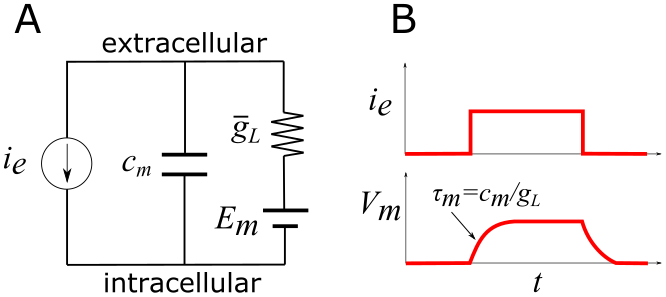
\includegraphics[width=0.8\textwidth]{Figures/Neuron/RCneuron.png}
\end{center}
\caption{\textbf{RC-neuron.}  A neuron model containing only a capacitive and a leakage current can be represented as an RC-circuit ($R = 1/g_L$). In the illustration, the neuron is given a current injection $I$ and responds by charging up the membrane. When the input is terminated, the membrane potential will return to the value $E_L$.
}
\label{Neuron:fig:RC}
\end{figure}

In the RC-model, $E_L$ will be identical to the resting potential of the neuron, i.e., the potential that the membrane will settle on in the case where it does not receive any input. In the more general models, which also include active ion channels (see below), the resting potential will still tend to be close to $E_L$, but will typically not be identical to $E_L$, as there some of the active ion channels can be partially open during rest, and thus affect the resting potential. For example values, see the parameters used in the original Hodgkin-Huxley model (Table \ref{tab:HH}).

\subsubsection{\blue{Active ion channels}}
In addition to $I_c$ and $I_L$, biophysical neuronal models typically include a number of active ion channels. In the HHC framework, current through an active an active ion channel $x$ is modeled as:

\begin{equation}
I_x = \bar{g}_x m_x^{\alpha} h_x^{\beta}(V-E_x).
\label{eq:HHform}
\end{equation}

Here, $\bar{g}_x$ (mS/cm$^2$) denotes the conductance when all channels of type $x$ are fully open (the bar indicates that it's a constant), while $E_x$ (mV) is the reversal potential for the ion species that travels through the channel. In analogy with the leak reversal potential, we may think of $E_x$ as the target potential that the current through ion channel $x$ will strive to drive the membrane potential towards. The intrinsic membrane potential dynamics is thus due to the competition between various currents that try to drive it towards their respective reversal potentials. We note that the current density $i_x$ does not represent the current through a single ion channel, but a large number of channels of the same type $x$. 

Active ion channels differ from the passive leakage channel in that their total conductance, $\bar{g}_{x} m^{\alpha} h^{\beta}$, will vary with time due to the so-called gating variables, in eq. \ref{eq:HHform} denoted $m$ and $h$. These determine the dynamics of how the ion channel activates or deactivates (opens or closes). Here, $m$ and $h$ represent two different types of gates, which have different dependencies in terms of what causes them to open/close. The exponents $\alpha$ and $\beta$ represent the number of copies that a channel $x$ has of each type of gate. The values of $m$ and $h$ interpret as the fraction of the gates of the various types that are open, and the values are thus numbers between 0 (all gates in the closed state) and 1 (all gates in the open state). For an ion channel to be open, all its gates must be in the open state. The product $m^{\alpha} h^{\beta}$ thus interprets as the fractions of ion channels that are open, so that the ion channel conductance is given by the product $\bar{g}_x m_x^{\alpha} h_x^{\beta}$.

For voltage-gated ion channels, the the dynamics of the gating variables can be described by kinetics equations on the form:
\begin{equation}
\frac{dx(\phi_m,t)}{dt} = \frac{x_{\infty}(\phi_m) - x}{\tau_x(\phi_m)},  \, \text{for } x = \{m,h\}.
\label{eq:HHgate}
\end{equation}
Here, the steady state activation $x_{inflty}(\phi_m)$, represents the fraction of gates that will end up in the open state if the cell is clamped at a given potential $\phi_m$ for sufficiently long time. However, the process of opening the gates takes some time, as represented through the activation time constant $\tau_x(\phi_m)$ (ms). Both $x_{inflty}(\phi_m)$ and $\tau_x(\phi_m)$ are functions of the membrane potential, and these must be determined experimentally for each individual ion channel type. We do not go into these experimental issues here, but will think of them as known functions. 

There are also many ion channels whose activation or inactivation does not depend on $\phi_m$, but on some other variable, such as the concentration of some ion species or ligand. A common example are Ca$^{2+}$ gated ion channels, i.e., channels with gate opening controlled by the intracellular Ca$^{2+}$ concentration ($[Ca^{2+}]_i$). There are also ion channels whose activation depend on more than one variable, such as e.g., ion channels whose activation depend on both $\phi_m$ and $[Ca^{2+}]_i$. Fortunately, a HHC type formalism can in most cases be applied also to these kind of ion channels, provided that $x_{inflty}(\phi_m)$ and $\tau_x(\phi_m)$ in eq. \ref{eq:HHgate} can be replaced with experimentally determined functions of the relevant variables. 

HH-type ion channels has become the gold standard for biophysically detailed neuronal simulations on the cellular and network level. Today, this framework is used for simulating the dynamics of large neuronal networks (see e.g., \cite{traub2005, markram2015, arkhipov2018}). It should be noted that HH-type ion channels are simplified approximations of the electrophysiological dynamics of ion channel gating, and ion channels could be modeled in greater detail, e.g. with Markov-type models (see e.g., \cite{Destexhe1994, balbi2017}). 


\subsubsection{\orange{Stimulus currents and synapses}}
Finally, the stimulus current in Eq. \ref{eq:singlecomp_zerosum}, can be represent any external stimulus that a neuron receives. Typically, it is either taken to represent an experimental current injection such as for example a step-current injection:

\begin{equation}
i_\text{inj}(x)= 
\begin{cases}
    constant, & \text{if } t_{start} > t > t_{end} \\
    0,              & \text{otherwise},
\end{cases}
\label{eq:injected}
\end{equation}
or a synaptic input. 

Synapses come in many forms, and they can be either inhibitory (making the receiving neuron less likely to fire) or excitatory (making the receiving neuron more likely to fire). The most common synapses are chemical synapses, which are normally modeled more or less like an ion channel:
\begin{equation}
I_\text{syn}(t) = g_\text{syn}(t) \big( \phi_m(t)-E_\text{syn} \big), 
\label{eq:chemicalsynapse}
\end{equation}
where $E_\text{syn}$ is the reversal potential of the synapse, and $g_\text{syn}(t)$ the conductance. Unlike for ion channels, which are often voltage or calcium activateD, the synapse is activated by neurotransmitters from the pre-synaptic cell. However, as the synaptic response tend to be quite stereotypical (i.e., it responds in the same way every time it is activated), it is common to model $g_\text{syn}(t)$ as a constant $\bar{g}_\text{syn}$ multiplied with a temporal kernel determining the opening and closing of a synapse set off at an activation time $t_s$. Typical choices for $g_\text{syn}(t)$ are: 

\begin{align}
&\text{(i) exponential decay:} \;\; g_\text{syn}(t) = \bar{g}_\text{syn} e^{-(t-t_\text{s})/\tau}\, \Theta(t-t_\text{s}) \\
&\text{(ii) $\alpha$-function:} \;\; g_\text{syn}(t) = \bar{g}_\text{syn} \frac{t-t_\text{s}}{\tau} e^{-(t-t_\text{s})/\tau} \, \Theta(t-t_\text{s}) \\
&\text{(iii) $\beta$-function:} \;\; g_\text{syn}(t) = \bar{g}_\text{syn} \frac{\tau_1 \tau_2}{\tau_1-\tau_2} 
\Big( e^{-(t-t_\text{s})/\tau_1} - e^{-(t-t_\text{s})/\tau_2} \Big) \, \Theta(t-t_\text{s}) \\
& \text{(iv)} g_\text{syn}(t) = \bar{g}_\text{syn} \frac{e^{-(t-t_\text{s})/\tau_1} - e^{-(t-t_\text{s})/\tau_2}} {1+\mu [\text{Mg}^{2+}] e^{-\gamma \phi_m} } \, \Theta(t-t_\text{s}),
\label{eq:synapseforms}
\end{align}
where $\Theta(t)$ is the (Heaviside) unit step function: $\Theta(t \ge 0)=1$,   $\Theta(t< 0)=0$. Simple waveform (cf., (i)--(iii) above) typically used for AMPA  and GABA receptors, while the waveform (iv), is mainly relevant for NMDA-receptors, 
where the conductance is influenced by membrane voltage and concentration of extracellular magnesium. In all these equation, $the \tau$'s and the $\gamma$ are parameters that determine the time course of the synapse opening, and must be tuned to experimental data. 

We should note that chemical synapses may be plastic, meaning that their maximum conductance $\bar{g}_\text{syn}$ can vary with time, depending on the spiking history of the neuron. Synaptic plasticity is the mechanism for learning and memory formation. We do not go further into this topic here. 

In addition to having chemical synapses, some neurons may also be connected directly by electrical synapses called \underline{gap junctions}, where the current from one neural process into the other is simply a function of the voltage difference between them and the conductance: 

\begin{equation}
i_\text{gap}=g_\text{gap} (\phi_{m2}-\phi_{m1})
\label{eq:gapjunction}
\end{equation}


\subsubsection{\orange{The Hodgkin-Huxley model}}
\ghnote{Maybe make this section as a box.}
To give an example of a model with active ion channels, we here list up the equations for the original Hodgkin-Huxley model. Compared to modern biophysically detailed neuron models, it is relatively simple in that it only contains two (voltage-gated) active ion channels, a Na$^+$ with three activation gates ($m^3$) and one inactivation gate ($h$), as well as a K$^+$ channel with four inactivation gates $n^4$:
\begin{equation}
c_m \frac{d\phi_m}{dt} = -\bar{g}_L(\phi_m-E_L) - \bar{g}_{Na} m^3 h (\phi_m - E_{Na}) - \bar{g}_{K} n^4 (\phi_m - E_{K}).
\label{eq:HHfull}
\end{equation}
The two active ion channels are together responsible for action potential generation. In eq. \ref{eq:HHfull}, $\bar{g}_{Na}$ and $\bar{g}_K$ are the conductances for fully open channels, while $E_{Na}$ and $E_{K}$ are the Na$^+$ and K$^+$ reversal potentials. Like we defined in eq. \ref{eq:HHgate}, the gating kinetics is given by: 
\begin{equation}
\frac{dx(\phi_m,t)}{dt} = \frac{x_{\infty}(\phi_m) - x}{\tau_x(\phi_m)},  \, \text{for } x = \{m,h,n\}.
\label{eq:HHgates}
\end{equation}
The experimentally determined functions for $x_{infty}(\phi_m)$ and $\tau_x(\phi_m)$, and all model parameter values are given in Table \ref{tab:HH}. An electric circuit representation of the HH model is depicted in Fig. \ref{Neuron:fig:HHcircuit}

\begin{table}[h!]
\begin{center}
\caption{The Hodgkin-Huxley model}
\label{tab:HH}
    \begin{tabular}{l}
    \hline
    $x_{\infty}(\phi_m) = \frac{\alpha_x(\phi_m)}{\alpha_x(\phi_m) + \beta_x(\phi_m)}$ for $x = m,n,h$ \\ \hline
    $ \alpha_n = \frac{0.01 \mathrm{ms}^{-1} \phi_m+55 \mathrm{mV}}{1-e^{-(\phi_m+55 \mathrm{mV})/10 \mathrm{mV}}}$  \\ \hline
    $ \beta_n = 0.125 \mathrm{ms}^-1 e^{-(\phi_m+65 \mathrm{mV})/80 \mathrm{mV}} $  \\ \hline
    $ \alpha_m = \frac{0.1 \mathrm{ms}^{-1} \phi_m+ 40 \mathrm{mV}} {1-e^{-(\phi_m+40 \mathrm{mV})/10 \mathrm{mV}}}$  \\ \hline
    $\beta_m = 4 \mathrm{ms}^{-1} e^{-(\phi_m+65  \mathrm{mV})/18 \mathrm{mV}} $  \\ \hline
    $\alpha_h = 0.07 \mathrm{ms}^{-1} e^{-(\phi_m+65 \mathrm{mV})/20 \mathrm{mV}}$  \\ \hline
    $\beta_h = \frac{1 \mathrm{ms}^{-1}}{1+e^{-(\phi_m+35 \mathrm{mV}))/10 \mathrm{mV})}} $  \\ \hline
    $c_m = 1.0 \mu $F/cm$^2$ \\ \hline
    $\bar{g}{Na} = 120\times 10^{-9}$ m$^2$/s\\ \hline
    $\bar{g}_{K} = 36$ mS/cm$^2$ \\ \hline
    $\bar{g}_{L} = 0.3$ mS/cm$^2$ \\ \hline
    $E_{Na} = 50$ mV \\ \hline
    $E_{K} = -77$ mV \\ \hline
    $E_{L} = -54.4$ mV \\ \hline
    \end{tabular}
\end{center}
\end{table}

\begin{figure}[!ht]
\begin{center}
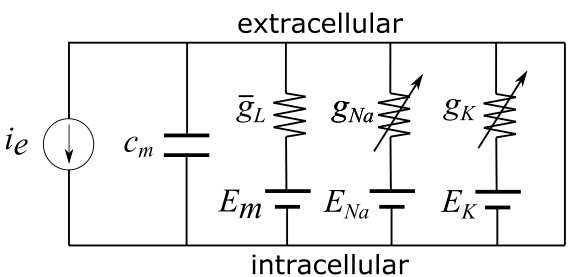
\includegraphics[width=0.8\textwidth]{Figures/Neuron/HHmodel.png}
\end{center}
\caption{\textbf{Hodgkin Huxley model.}
}
\label{Neuron:fig:HHcircuit}
\end{figure}



%%%%%%%%%%%%%%%%%%%%%%%%%%
\subsection{\blue{Morphology}}
The formalism introduced so far has been for the modeling a neuron as a single compartment. When doing that, one implicitly assumes that the whole neuron is isopotential (same $\phi_m$ evenrywhere). This is generally not true, and especially not in neurons with long and branchy dendrites, where $\phi_m$ can be very different in the soma compared to what it is in the tip of a distal dendrite. Models that account for morphological features of neurons are called multicompartmental models (Fig. \ref{Neuron:fig:multikompisen}A). The neural morphology is then represented as cylindrical compartments connected with resistors, and $\phi_m$ can be computed in each individual compartment. 

\begin{figure}[!ht]
\begin{center}
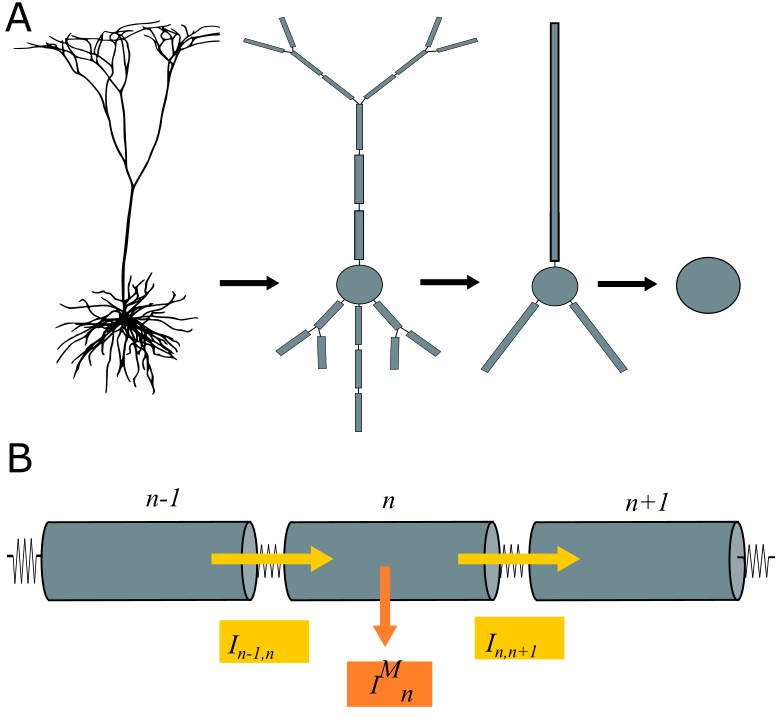
\includegraphics[width=0.7\textwidth]{Figures/Neuron/Multikompis.png}
\end{center}
\caption{\textbf{Multi-compartment model.} {\bf (A)} Representations of a neuronal morphology as a number of interconnected compartments. {\bf (B)} Subset of interconnected compartments. The currents involved in multicompartmental modelling include the sum of transmembrane currents ($I^M_n$) in a compartment $n$, and the intracellular currents running between 
compartments, $I_{n-1,n}$ (current from compartment $n-1$ to $n$), and $I_{n,n+1}$ (current from compartment $n$ to $n+1$).}
\label{Neuron:fig:multikompisen}
\end{figure}

As a simple introduction to the formalism used in HHC-type models, let us consider a subset of three connected cylindrical compartments which we number $n-1$, $n$ and $n+1$( Fig. \ref{Neuron:fig:multikompisen}B). Let us for simplicity assume that the three cylinders have the same length ($L$) and diameter ($d$). The two categories of currents that run in this system are (i) the transmembrane currents that we introduced in the previous subsection, all of which we can group together into a total transmembrane current $I^M_n$, and (ii) the axial currents running between the cylindrical compartments ($I_{n-1,n}$ and $I_{n,n+1}$). The dynamics of this system is computed using Kirchhoff's current law, which demands that the sum of currents into a given segment ($n$) should be zero:

\begin{equation}
I_{n-1,n} - I_{n,j+1} - I^M_n = 0
\label{eq:Kirch}
\end{equation}
We note that we calculate with total currents here (unit A), not current densities. The axial currents between two compartments are proportional to the voltage difference between the compartments, as determined by Ohms law:
\begin{eqnarray}
I_{n-1,n} = \frac{\phi_{n-1}-\phi_n}{4 R_a L/(\pi d^2)}, \nonumber \\ 
I_{n,n+1} = \frac{\phi_{n}-\phi_{n+1}}{4 R_a L/(\pi d^2)}.
\label{eq:axialcurrents}
\end{eqnarray}
Here, the denominators represent the axial resistance between two compartments, defined in terms of the axial resistivity $R_a$ ($\Omega$ cm), a material property of the cytosol solution, the cross section area $\pi d^2/4$, and the segment length or travel distance ($L$ (m)). We note that $\phi_n$ is the \emph{intracellular} potential in compartment $n$, but we shall in the reminder of this chapter assume that the extracellular space is isopotential and grounded ($\phi = 0$ there), so that the $\phi_n$ will be identical to the membrane potential in compartment $n$.

It should be noted that the situation becomes more complicated when the connected cylinders are of different length and diameter, and especially at branch points. However, the theory for computing the dynamics in branching structures with varying diameters is well established \cite{Rall1977,Rall1989}, and designated software such as NEURON \cite{Hines1997, Hines2009} automatizes the compartmentalization for the user once the neural morphology is specified. It should also be noted that the HHC formalism assumes that the neuronal morphology is well represented by a one-dimensional, branching cable, meaning that radial components of intracellular currents are neglected (see e.g.,\cite{lindsay2004maxwell} for a critical study of this approximation). 

For the reminder of this chapter, we limit ourselves to consider the simplified, unbranched scenario (Fig. \ref{Neuron:fig:multikompisen}B), as we deem this as sufficient for establishing an understanding of the essentials of morphology modeling. 


%%%%%%%%%%%%
\subsubsection{\blue{Active multicomparmtent models}}
To specify our HHC-type neuron model further, we write out the total membrane current as:
\begin{equation}
I^M_n = I_n^{cap} + I_n^{ion} + I_n^{stim} = -\pi d L c_m \frac{d\phi_n}{dt} + \pi d L i_n^{ion} + I_n^{stim}, 
\label{eq:Imemb}
\end{equation}
where $I_n^{ion}$ represent the total current density of all transmembrane ionic currents through leakage and active ion channels. On the right hand side, we have expressed the capacitive and ionic currents (mA) as current densities (mA/cm$^2$) multiplied with the membrane area ($\pi d L$ (cm$^2$)) represented by the sides of the cylinder. If we insert this into Eq. \ref{eq:Kirch}, we get:

\begin{equation}
c_m \frac{d\phi_n}{dt} = i_n^{ion} + \frac{d}{4R_a}\left(\frac{\phi_{n+1}-\phi_n}{L^2} - \frac{\phi_n-\phi_{n-1}}{L^2} \right) + \frac{I^{stim}}{\pi d L}.
\label{eq:multimain}
\end{equation}
Here,  $i_n^{ion}$ can contain any combination of passive and active membrane mechanisms. For whatever choice of membrane mechanisms, Eq. \ref{eq:multimain} can be solved numerically for appropriately chosen boundary conditions, the most common being to use either a sealed end ($\frac{\partial \phi_n}{\partial x} = 0$), or a killed end ($\phi_n=0$). The NEURON simulator by default uses the sealed-end condition, which means that no axial current leaves at the ends of the simulated structure. Eq. \ref{eq:multimain} is the fundamental equation for multicompartmental models.


%%%%%%%%%%%%%%%%%
\subsubsection{\blue{Passive multicompartment models}}
In the case when we have no active ion channels, $i_n^{ion} = g_L(\phi_n - E_L)$ is simply the leakage current density. In purely passive models, it is custom to refer to the leakage reversal potential simply as the membrane resting potential, and call it $E_m$. It is also custom to replace the leak conductance $g_L$ with the membrane resistivity $R_m = 1/g_L$ ($\Omega$ cm$^2$). Eq. \ref{eq:multimain} then simplifies to:

\begin{equation}
c_m \frac{d\phi_n}{dt} = \frac{E_m-\phi_n}{R_m} + \frac{d}{4R_a}\left(\frac{\phi_{n+1}-\phi_n}{L^2} - \frac{\phi_n-\phi_{n-1}}{L^2} \right) + \frac{I^{stim}}{\pi d L}
\label{eq:multipassive}
\end{equation}

Although all neurons contain some active membrane mechanisms, the passive model (Eq. \ref{eq:multipassive}) is still often used as an approximation for signaling in neural dendrites, which tend to have a lower density of active mechanisms compared to the soma and axon. 


%%%%%%%%%%%%%%%%%%%%
\subsubsection{\blue{Cable equation}}
If we in Eq. \ref{eq:multipassive} let $L \rightarrow \delta x$, and take the limit $\delta x \rightarrow 0$, we may derive the cable equation (see e.g., \cite{Sterratt2011}): 

\begin{equation}
c_m \frac{\partial \phi}{\partial t} = \frac{E_m-\phi}{R_m} +  \frac{d}{4 R_a}  \frac{\partial^2 V}{\partial x^2}  + \frac{I_e}{\pi d},
\label{eq:cable}
\end{equation}
where we have introduced the stimulus current per unit length, $I_e(x,t) = I^{stim}/\delta x$ (mA/cm). To improve our analytical understanding of dendritic signaling, it is useful to reformulate the cable equation to:
\begin{equation}
\tau_m \frac{\partial \phi}{\partial t} = E_m-\phi +   \lambda^2  \frac{\partial^2 \phi}{\partial x^2}  + \frac{I_e R_m}{\pi d},
\label{eq:cable2}
\end{equation}
where we have introduced the length constant,
\begin{equation}
\lambda = \sqrt{\frac{d R_m}{4 R_a}} \,\, \text{cm}, 
\label{eq:lengthconst}
\end{equation}
and the time constant, 
\begin{equation}
\tau_m \equiv R_m c_m  \,\, \text{ms}.
\label{eq:timeconst}
\end{equation}
The cable equation serves as a continuous version of a passive neural branch (with infinitely many infinitely small compartments), 
where $\tau_m$ is typical time scale (dimensionless time: $t/\tau$), while $\lambda$  is typical length scale  (dimensionless time: $x/\lambda$) for signals in the cable. If a certain point along the cable is set to a certain potential $\phi$, $\tau_m$ will tell us how fast this local potential will dissipate towards rest, while $\lambda$ will tell us how long part of the cable that will be affected by this local potential. 

Whereas multicompartmental models (Eq. \ref{eq_multimain} and \ref{eq:multipassive}) generally must be solved numerically, the cable equation allows the spatiotemporal evolution of the membrane potential to be solved numerically for some idealized scenarios. Below, we consider a couple of scenarios that will also make the interpretation of $\tau_m$ and $\lambda$ clearer. 


%%%%%%%%%%%%%%%%%%%%
\subsubsection{\orange{Steady state solution of the cable equation}}
As an example solution, we consider the steady state solution of a semi-infinite cable, receiving a constant current injection $I_e$ at the sealed end in $x=0$ (Fig. \ref{fig_Semiinf}).

\begin{figure}[!ht]
\begin{center}
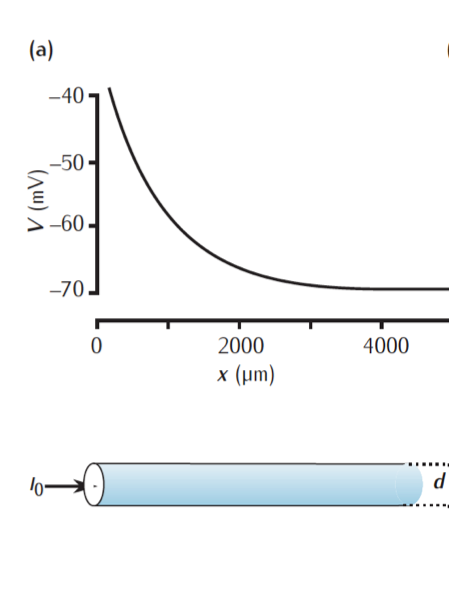
\includegraphics[width=0.7\textwidth]{Figures/Neuron/Semiinf.png}
\end{center}
\caption{\textbf{Semi-infinite cable receiving input $I_e$ in sealed end at $x=0$.} Parameters are $d = 1$ $\mu$m, $R_a=35.4$ cm, $R_m = 10$ m$\Omega$cm$^2$, which gives a length constant $\lambda = 840\, \mu$m. }
\label{Neuron:fig:Semiinf}
\end{figure}

At steady-state, Eq. \ref{eq:cable2} becomes:
\begin{equation}
0 = E_m-\phi_m +  \lambda^2 \frac{\partial^2 \phi_m}{\partial x^2}, 
\label{eq:semiinf}
\end{equation}
at all points along the cable, except $x=0$, where there is the additional injected current, which we will deal with later. If we introduce the new variable $\Delta{phi_m}=\phi_m-E_m$, Eq. \ref{eq:semiinf} simplifies to:
\begin{equation}
\frac{d^2 \Delta{\phi_m}}{d x^2} -  \frac{1}{\lambda^2} \Delta{\phi_m}=0, 
\label{eq:semiinf2}
\end{equation}
which has the solution:
\begin{align}
\Delta{\phi_m}(x) &= \Delta{\phi_m}(0) e^{-x/\lambda} \\
\phi_m(x) &= E_m + \big( \phi_m(0)-E_m \big) e^{-x/\lambda}.
\label{eq:semiinf3}
\end{align}
The general-solution to the equation also has a term containing $e^{+x/\lambda}$, but this was excluded from the solution on the count of being unphysical as it diverges when $x \rightarrow \infty$.The injected current will determine what $\phi_m(0)$ is a the boundary, and we may introduce it by defining the input resistance in steady state as $R_{\infty} =  \Delta \phi_m/I_e =  (\phi_m(0)-E_m)/I_e$, according to Ohm's law. With this, Eq. \ref{eq:semiinf3} can be written:
\begin{equation}
\phi_m(x) = E_m + R_{\infty} I_e e^{-x/\lambda}
\label{eq:semiinf4}
\end{equation}

Eq. \ref{eq: semiinf4} is useful as it gives us analytical insight into signals spreading in e.g., passive dendrites. It tells us that in steady-state, the amplitude will decay exponentially from the injection site and outwards, and will be reduced by a factor $1/e$ over the length $\lambda$. If we put in some typical values in eq. \ref{eq:lengthconst}, like a dendritic diameter $d=1$~$\mu$m, a membrane resistance of $R_m=10\;\text{k}\Omega\text{cm}^2$, and an axial resistivity $R_a=35.4\;\Omega\text{cm}$, we would get a length constant of $\lambda = 840\; \mu$m. 

Eq. \ref{eq:lengthconst} also sows that $\lambda \propto \sqrt{d}$, meaning that signals will spread further the thicker the dendrite, and that $\lambda \propto \sqrt{R_m/R_a}$ meaning that the signal is facilitated by having a large membrane resistance compared to the axial resistance. We may also get some insight in what aspects of the neurite that determine the input resistance $R_{\infty}$ by requiring that the axial current at $x=0$ should be identical to the input current. From that, we can calculate the input resistance, 

\begin{align}
&- \frac{4R_a}{\pi d^2} \frac{\partial \phi_m}{\partial x}  = i_e  \Big|_{x=0} \\
&\frac{4R_a \lambda}{\pi d^2} R_{\infty} i_e  = i_e \\
&R_{\infty} =  \sqrt{\frac{4R_m R_a}{\pi^2 d^3}}, 
\label{eq:inputresistance}
\end{align}
where we used eq. \ref{eq:semiinf3} for $\phi_m$ and eq. \ref{eq:lengthconst} for $\lambda$. Eq. \ref{eq:inputresistance} shows that the input resistance is proportional to $1/d^{3/2}$, i.e., the input resistance is higher the thinner the dendrite. 


\subsubsection{\blue{Frequency dependence of the cable length constant}}
As we just saw, the length constant $\lambda$ (eq. \ref{eq:lengthconst}) is the length over which the potential falls to a fraction $1/e$ of its boundary value when the finite end of a semi-infinite cable is fixed at a constant potential. As this interpretation depends on a constant, direct-current (DC), boundary condition, $\lambda$ is often referred to as the DC length constant. 

It is possible to derive a corresponding length constant for AC input to a semi-infinite cable \cite{Pettersen2008a}: 
\begin{equation}
\lambda_{AC} = \lambda \sqrt{ \frac{2}{1+\sqrt{(\omega \tau)^2 + 1}} }.
\label{eq:AClambda}
\end{equation}
Here $\tau$ still is the membrane time constant (eq. \ref{eq:timeconst}), $\lambda$ is still the DC length constant (eq. \ref{eq:lengthconst}), and $\omega = 2\pi f$ is the angular frequency of the the boundary potential.

For a constant boundary condition ($I_e = \text{constant}$ in eq. \ref{eq:semiinf4}) or, equivalently, $\phi_m(0) = \text{constant} in eq. \ref{eq:semiinf3}), $\omega$ is zero, and we may verify that $\lambda_{AC}$ becomes identical to the DC length constant $\lambda$. For an AC input, we see that $\lambda_{AC}$ decreases with $\omega$, and for high frequencies $\lambda_{AC} \propto (\omega \tau^{-1/2})$. Thus, low frequency input will tend to travel further in dendritic structures, while high frequency input will affect dendritic structures more locally. 

As we shall see later, an important factor determining the size and shape of extracellular potentials is the distance between inward (sinks) and outward (sources) transmembrane currents. This spatial separation is proportional to the neuronal length constant, and from eq. \ref{eq:AClambda} we thus know that the source/sink separation will be larger for low frequency components of the neuronal activity.


\subsubsection{\orange{Temporal solutions of cable equation}}
It can be shown that the temporal solution for $\phi_m$ in a passive cable is \cite{rall1969}:
\begin{equation}
\phi_m(x,t) = C_0(x) e^{-t/\tau_0} + C_1(x) e^{-t/\tau_1} + C_2(x) e^{-t/\tau_2} + \ldots, 
\label{eq:cabletemporal}
\end{equation}
where the coefficients $C_n(x)$ depend on the distance along the cable, while $\tau_0 = \tau_m = R_m C_m$ is the \emph{membrane time constant} (eq. \ref{eq:timeconst}), and the other time constants have successively smaller values ($\tau_0 > \tau_1 > \tau_2 > \ldots$). Fig. \ref{Neuron:fig:temporalrall} shows the the membrane potentials at selected positions along a $500 \, \mu$m long cable responding to a current injection (top panel) resembling a synaptic input in one end. We see that the peak response comes faster in proximal than in distal location, but that potential is about the same at all points along the cable after 2 ms. After this, $\phi_m$  decay gradually towards the resting state. This decay takes place at the slower time scale of the membrane time constant, which in this simulation was 10~ms ($R_m=1\,\Omega \text{m}^2$, and $C_m=1\,\mu\text{F}/\text{cm}^2$). Although the dynamics of course will be system specific, depending on the membrane time constant and generally on the presence of active mechanisms, the simulation in Fig. \ref{Neuron:fig:temporalrall} may give some general idea on how signals spread in dendrites.

\begin{figure}[!ht]
\begin{center}
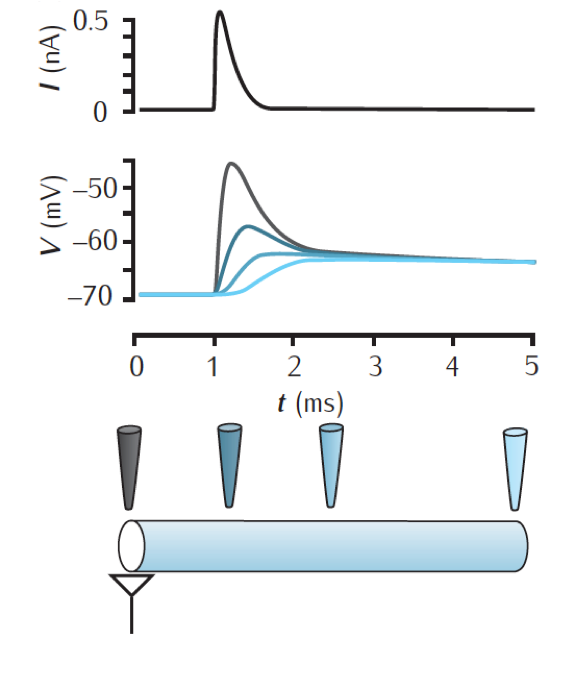
\includegraphics[width=0.7\textwidth]{Figures/Neuron/Temporalcable.png}
\end{center}
\caption{\textbf{Temporal solution of cable equation.}
}
\label{Neuron:fig:temporalrall}
\end{figure}


%%%%%%%%%%


\subsection{\orange{Ion concentration dynamics and reversal potentials}}
Action potentials are generated by a transmembrane influx of Na\textsuperscript{+}, which charges up (depolarizes) the neuron, 
followed by an efflux of K\textsuperscript{+}, which decharges (repolarizes) it. These fluxes are primarily driven by diffusion, and thus depend on the intra- and extracellular solutions having different ionic compositions. Neurons possess a set of homeostatic mechanisms that strive to maintain the trans-membrane ion concentration gradients. The perhaps most important is the ATPase pump, which uses energy to pump K$^+$ ions into the neuron and Na$^+$ ions out, and as a result, the intracellular space tends to remain comparatively rich in K$^+$, while the extracellular space is tends to remain comparatively rich on Na$^+$. Typical values of ion concentrations of the main charge carriers inside and outside neurons are given in Table \ref{table:ion-concentrations}. 


\begin{table}[h]
\centering
\caption{Major charge carrier concentrations inside/outside a typical mammalian neuron. Example values taken from \cite{Wu2019}, but may vary with species and brain regions. Nernst potentials were computed from Eq. \ref{eq:revpots} assuming a body temperature of 309.15 K.}
\label{table:ion-concentrations}
{\begin{tabular}{lccccc}\toprule
						    & 	K$^+$	&	Na$^+$	&	Mg$^2+$	  &	Cl$^-$	&	Ca$^{2+}$	 \\ \midrule
Inside (mM)				    & 140		&		10	&		0.5	&	10		&  	10$^{-4}$	  	\\
Outside (mM)			           & 5			&		145	&		2	&	110 		&		2		  	\\
Nernst potential (mV)		    &	-89		&	    	+71	&		+19	&	-64		&		+132 		  	\\
\bottomrule
\end{tabular}}{}
\end{table}

In the HHC-type formalism presented in this chapter, ion concentrations were implicitly assumed to be constant, and they did therefore not enter into the equations. As neuronal electrodynamics is generated by ions crossing the membrane, this may seem like a peculiar assumption. The reason why it is often fairly good, is that the number of ions crossing the membrane during a brief signal such as an action potential only leads to minor changes in the ion concentrations on either side of the membrane, so that concentrations changes on a short time scale can be neglected. On the longer time scale, the ATPase pump, and a set of other homeostatic mechanisms,  typically succeed in restoring baseline concentrations. In HHC-type models, the ensemble of processes that work to maintain baseline conditions are therefore not explicitly modeled, but are grouped into the \textit{passive} leakage current $I_L$ (eq. \ref{eq:HHleak}), which largely determines the cell's resting potential (see see \cite{offner1991} for a critical study of this approximation).

Below, we shall explain how the ionic concentrations are implicitly present in the HHC-formalism as they determine the ionic reversal potentials ($E_x$ in eq. \ref{eq:HHform}). We shall also comment on the cases where the assumptions of constant ion concentrations are not applicable. 


\subsubsection{Ionic reversal potentials}
Ion channels are pores in the membrane, some of which are selectively permeable only to specific ions. For example, when a Na$^+$ channel opens, Na$^+$ ions will diffuse from the extracellular space, where the Na$^+$ concentration is highest, and into the neuron. As this diffusive process transfers charged ions into the neuron, it will increase (depolarize) the membrane potential. The increased potential will in turn evoke an electrostatic force on the Na$^+$ ions, causing an electrical drift of Na$^+$ in the opposite (outward) direction. 

The ionic reversal potential is defined as the membrane potential at which the electrical drift current and diffusive current of a given ion species are in an equilibrium, i.e., they are equal in magnitude but oppositely directed. It can be calculated from the Nernst-Planck equation for electrodiffusion. If we approximate the problem as one-dimensional (in the $z$-direction, perpendicular to the membrane), the Nernst-Planck equation for an ion species $k$ is:

%%%%
\begin{equation}
j_k = j_{k,\text{diff}} + j_{k,\text{drift}} 
=  - P_k \Big(\frac{d[k]}{dz} +  \frac{Fz_k}{RT}  [k] \frac{d\phi}{dz} \Big), 
\label{eq:NP1D}
\end{equation}
%%%%
where the first term is Fick's law for the diffusive flux density along the concentration gradient, and the second term is the electrical drift along the voltage gradient. Here, the membrane's permeability ($P_k$) to ion $k$ has taken the role of the diffusion constant ($D_k$) which appears in the more common form of the Nernst-Planck equation. Furthermore, $z_{k}$ is the valency of ion species $k$, $R = 8.314$ J mol$^{-1}$K$^{-1}$ is the gas constant, $F = 96485.3365$ C/mol is Faraday's constant, and $T$ is the absolute temperature (K). The reversal potential (also called the Nernst-potential) is found by solving for when there is no net flux, i.e., when  $j_{k,\text{diff}} = - j_{k,\text{drift}}$:

\begin{equation}
\frac{1}{[k]} \frac{d[k]}{dz} = - \frac{Fz_k}{RT}  \frac{d\phi_m}{dz}.
\end{equation}
We may multiply both sides by $dz$ and re-arrange this to get:
\begin{equation}
-d\phi = \frac{RT}{Fz_k}  \frac{d[k]}{[k]}.
\end{equation}
Now we may integrate from the inside to the outside of the membrane:
\begin{align}
-\int_{\phi_{\text{in}}}^{\phi_{\text{out}}}  dV &= \frac{RT}{Fz_k}  \int_{[k]_{\text{in}}}^{[k]_{\text{out}}} \frac{d[k]}{[k]} \rightarrow \\
\phi_{\text{in}}-\phi_{\text{out}} &= \frac{RT}{Fz_k} ln \frac{[k]_{\text{out}}} {[k]_{\text{in}}} \rightarrow \\
E_k & =  \frac{RT}{Fz_k}  ln \frac{[k]_{\text{out}}} {[k]_{\text{in}}} 
\label{eq:revpots}
\end{align}
where the last equality follows from the definition of $E_k$ as the membrane potential $\phi_{\text{in}}-\phi_{\text{out}}$ for which the the net flux (in Eq. \ref{eq:NP1D}) is zero. Eq. \ref{eq:revpots} was used to compute the reversal potentials listed in Table \ref{table:ion-concentrations}. As ion concentrations are generally assumed to remain constant in HH-type models, the reversal potentials are also assumed to be constant. As a consequence, one typically do not think about ionic concentrations when constructing such models, but simply use values for $E_k$ based or empirical measurements of the potential at which a certain ion current becomes zero.

Eq. \ref{eq:NP1D} defined the reversal potential for an individual ion species, which is relevant for ion specific ion channels. In contrast, the passive membrane has some leakage permeability to all ion species simultaneously. This gives rise to a leak reversal potential $E_L$ (from Eq. \ref{eq:HHleak}), representing the equilibrium condition where the leakages of various ions across the membrane sum to a zero net electrical current.  If we assume that only the three most important charge carriers (K$^{+}$, Na$^{+}$ and Cl$^{-}$) contribute, and that they have leak permeabilities $P_K$, $P_{Na}$ and $P_{Cl}$, it can be shown that they are in equilibrium at the potential:

\begin{equation}
E_L = \frac{R T}{F} 
\ln \frac{P_\text{K} [K]_\text{out}+P_\text{Na} [Na]_\text{out} + P_\text{Cl} [Cl]_\text{in}}
           {P_\text{K} [K]_\text{in}+P_\text{Na} [Na]_\text{in} + P_\text{Cl} [Cl]_\text{out}}.
\label{eq:Eleak_GHK}
\end{equation}


\subsubsection{The Goldman-Hodgkin-Katz equation}
If one combines Eq. \ref{eq:NP1D} with the assumptions that (i) ions cross the membrane independently, and (ii) that the electrical field within the membrane is constant, one can derive the Goldman-Hodkgkin-Katz (GHK) equation for the membrane currents (see e.g., \cite{hodgkin1949, johnston1994foundations}):

\begin{equation}
I_\text{k} = P_k z_k F \frac{z_k F \phi_m}{R T} \Big( \frac{[k]_\text{in}-[k]_\text{out} e^{-z_k F \phi_m/RT}} {1-e^{-z_k F \phi_m/RT}} \Big).
\label{eq:GHK}
\end{equation}

Looking at eq. \ref{eq:GHK}, we see that the transmembrane currents are nonlinear functions of both the ionic concentrations $[k]$ in the intra and extracellular space, and the membrane potential $\phi_m$. In comparison, the transmembrane currents used in the HH-type formalism (eq. \ref{eq:HHform}), which are proportional to the driving force $(V-E_k)$, are linearized (sometimes called quasi-Ohmic) versions of the Goldman-Hodkgkin-Katz equation. The HH-form (eq. \ref{eq:HHform}) is generally deemed as sufficient for modeling most ion channels, because it gives good predictions of the membrane currents. Ion concentrations are then not modeled, and ionic reversal potentials are assumed to be constant. 

The leakage reversal potential (eq. \ref{eq:Eleak_GHK}) can be derived from eq. \ref{eq:GHK} by requiring that the sum of all ionic currents, each independently defined by eq. \ref{eq:GHK}, is zero.


\subsubsection{Intracellular  Ca\textsuperscript{2+} dynamics}
While ion concentrations are typically assumed to be constant in HHC-based models, it is common to make an exception for Ca\textsuperscript{2+}. The main reason for this is that the intracellular Ca\textsuperscript{2+} concentration ($\text{[Ca]_i}$) is very low compared to that of the other ion species (Table \ref{tab:HH}). Unlike for the other ion species,  $\text{[Ca]_i}$, can therefore change quite dramatically on a short time scale, e.g., during the opening of Ca\textsuperscript{2+} channel. 

The motivations for modeling $\text{[Ca]_i}$ are several. Firstly, to accurately model currents through Ca\textsuperscript{2+} channels, the concentration dependent GHK formalism (eq. \ref{eq:GHK}) is often used (see e.g., \cite{Destexhe1994, Zhu1999, Halnes2011}). Secondly, Ca\textsuperscript{2+} does not only act as a charge carrier in neurons, but is also a second messenger, which means that it can trigger a number of intracellular chemical processes, including the gating of Ca\textsuperscript{2+} activated ion channels. Thirdly, modeling $\text{[Ca]_i}$ could be motivated by the aim to reproduce data from Ca\textsuperscript{2+} imaging experiments. 

When Ca\textsuperscript{2+} dynamics is included in HHC-based models of the electrical activity of neurons, it is usually to account for the activation of ion channels that instead of being voltage gated, open or close as a function of $\text{[Ca]_i}$. The kinetics scheme for voltage gated ion channels (\ref{eq:HHgate}) is then replaced with one dependent on $\text{[Ca]_i}$:

\begin{equation}
\frac{dx(\phi_m,t)}{dt} = \frac{x_{\infty}(\text{[Ca]_i}) - x}{\tau_x(\text{[Ca]_i}},  \, \text{for } x = \{m,h\},
\label{eq:Cagate}
\end{equation}
and the $\text{[Ca]_i}$ in a neuronal compartment is typically modeled using a simplified framework on the form:
\begin{equation}
\frac{d\text{[Ca]_i}}{dt} = \gamma i_{Ca} - \frac{\text{[Ca]_i}-\text{[Ca]_{i,0}}}{\tau_{Ca}}, 
\label{eq:Cadynamics}
\end{equation}
where a transmembrane Ca\textsuperscript{2+} current ($i_{Ca}$ is converted to a change in $\text{[Ca]_i}$ by the conversion factor $\gamma$, which is proportional to the surface to volume ratio of the neuronal compartment where $\text{[Ca]_i}$ is defined. In addition, the last term in eq. \ref{eq:Cadynamics} represents the summed activity of a number of extrusion mechanisms that will make $\text{[Ca]_i}$ will decay towards some baseline value $\text{[Ca]_{i,0}}$ with a time constant $\tau_{Ca}$ (see e.g. \cite{Sterratt2011}).



\subsection{\orange{Underlying assumptions in the Hodgkin-Huxley-Cable framework}}
As the final part of this chapter, we will discuss two important assumptions that the HHC-framework was based upon, namely that (i) the concentrations of the main charge carriers (K$^{+}$, Na$^{+}$ and Cl$^{-}$) are constant, and (ii) that the extracellular space is isopotential and grounded, so that the extracellular potential ($\phi_e$) is zero there. 



\subsubsection{Constant ion concentrations}
In most neuronal models based on the HHC framework, the reversal potentials (eq. \ref{eq:revpots}) of the main charge carriers are assumed to be constants, which implicitly means that ion concentrations are assumed to be constant. If this were not true, and 
so that the ion concentrations and reversal potentials were allowed to change, it could potentially have a dramatic impact on the neurodynamics. 

As we saw earlier (eq. \ref{eq:Cadynamics}) some models do indeed account for Ca\textsuperscript{2+} dynamics, and it could seem natural to think that one might use a similar framework for all the other ion species as well. A simple reason for not doing this is, as we have stated, that there is no motivation for it because they change so little during normal activity. A more complex reason is a framework equivalent to that in eq. \ref{eq:Cadynamics} might not be all that meaningful for the more abundant ion species, as we shall explain below. 

Another reason is that it might not be all that m


However, the simple model for ion concentration dynamics given by eq. \ref{eq:Cadynamics} rests on some important approximations.
Firstly, the model is local in the sense that $\text{[Ca]_i}$ changes as a function of the transmembrane flux only. Intracellular diffusion and electrical migration of Ca\textsuperscript{2+} are thus assumed to have a negligible impact on the dynamics of $\text{[Ca]_i}$. In principle, such electrodiffusive processes could have an impact both on the dynamics of $\text{[Ca]_i}$ and on the dynamics of the membrane potential, since diffusing ions will carry electrical currents (see e.g., \cite{Qian1989}). 

Secondly, the model represented by eq. \ref{eq:Cadynamics} is not ion conserving, since it allows $\text{[Ca]_i}$ to change inside the neuron without the extracellular Ca\textsuperscript{2+} concentration changing accordingly. This approximation may work fairly well for Ca\textsuperscript{2+}, since the intracellular concentration is so much lower than the extracellular. For other ion species, intra- and extracellular concentrations are of more comparable magnitudes, and for these it might not be meaningful to model the intracellular concentration without also modeling the extracellular concentrations. 

To model the extracellular ion concentrations, one needs to define extracellular compartments of finite volumes, either by making some simplified approximation that each intracellular compartment has a (single) finite extracellular compartment to its disposal (see e.g., \cite{Kager2000, kneller2002, Cressman2009, WeiUllahSchiff2014, Saetra2020}), or by meshing up the extracellular space and computing the ion concentration dynamics there using some numerical framework for diffusion (see e.g., \cite{newton2018}) or electrodiffusion (see e.g., \cite{ellingsrud2020}). Such frameworks are generally computationally heavy, and can not be based on the simplified HHC scheme presented in this chapter. 

Generally, it is believed that ion concentrations change little during normal neuronal activity, so that the HHC-type framework works well. However, many pathological conditions, including epilepsy and spreading depression, are associated with dramatical shifts in extracellular concentrations \cite{Somjen2001, Zandt2015, Ayata2015}, and alternative frameworks could be considered for modeling such scenarios. We shall revisit the topic of extracellular ion concentration dynamics in chapter \ref{sec:Eldiff}.







\subsection{\orange{Effects of extracellular potentials on neurodynamics}}
In the remainder of this book, the focus will on the extracellular potential ($\phi_e$). The motivation for introducing the HHC formalism is that HHC-based neuron models are a common starting point when one wants to simulate $\phi_e$. 

In forward modeling of $\phi_e$, the workflow typically includes two steps. First, one computes all neuronal transmembrane currents in an independent simulation based on the HHC formalism. Next, one uses volume conductor theory, as we will present in the next chapter (chapter \ref{sec:VC}), to estimate the extracellular potential evoked by these currents. This approach has an evident inconsistency: The fundamental equation the HHC formalism (eq. \ref{eq:multimain}) was derived under the assumption that the extracellular space is isopotential and grounded. Hence, one uses neuron models based on the assumption that $\phi_e = 0$ to later predict a nonzero $\phi_e$. 

Despite this inconsistency, the approach often give fairly accurate results. The reason is that $\phi_e$ tends to be much smaller than the membrane potential $\phi_m$


The approximation is nevertheless useful since $\phie$ is typically so much smaller than $\phim$ that the (ephaptic) effect of $\phie$ on neurodynamics can be neglected without severe loss in accuracy \cite{anastassiou2015}. 



\begin{equation}
I_{n-1,n} - I_{n,j+1} - I^M_n = 0
\label{eq:Kirch}
\end{equation}
We note that we calculate with total currents here (unit A), not current densities. The axial currents between two compartments are proportional to the voltage difference between the compartments, as determined by Ohms law:
\begin{eqnarray}
I_{n-1,n} = \frac{\phi_{n-1}-\phi_n}{4 R_a L/(\pi d^2)}, \nonumber \\ 
I_{n,n+1} = \frac{\phi_{n}-\phi_{n+1}}{4 R_a L/(\pi d^2)}.
\label{eq:axialcurrents}
\end{eqnarray}
Here, the denominators represent the axial resistance between two compartments, defined in terms of the axial resistivity $R_a$ ($\Omega$ cm), a material property of the cytosol solution, the cross section area $\pi d^2/4$, and the segment length or travel distance ($L$ (m)). We note that $\phi_n$ is the \emph{intracellular} potential in compartment $n$, but we shall in the reminder of this chapter assume that the extracellular space is isopotential and grounded ($\phi = 0$ there), so that the $\phi_n$ will be identical to the membrane potential in compartment $n$.

\subsection{\red{Utklipp}}
The HH-type framework does have some limitations. Firstly, HH-type ion channel models (cf. eq.\ref{eq:HHform}) are somewhat crude representations of the electrophysiological dynamics of single ion channel gating, and alternative models exist which models ion channels in greater detail, e.g. with Markov-type models (see e.g., \cite{Destexhe1994, balbi2017}). SThirdly, in HH-type models, ion concentrations of the main charge carriers are assumed to remain effectively constant under the simulated period. Fourthly, the extracellular potential is assumed to be constant and grounded, so that it does not provide any (ephaptic) feedback effects on the computed neurodynamics. 

The two first of the above listed assumptions regard the level of detail in the representation of the neuron.

the two latter regard the interaction between the neuron and its surroundings, and thus the physical consistency of the modeling framework. As the two latter assumptions are most relevant for the interplay between the neurodynamics and extracellular potentials, we shall pay some extra attention to those.





The HH-type framework presented in this chapter, has become the gold standard for biophysically detailed neuronal simulations on the cellular and network level. Today, this framework is used for simulating the dynamics of large neuronal networks (see e.g., \cite{traub2005, markram2015, arkhipov2018}). 









Neuronal modeling as presented here, based on the combination of a Hodgkin-Huxley type formalism for membrane mechanisms, and cable theory for intracellular signal propagation, is the standard framework for biophysical modeling of neurodynamics at the cellular and network level  \ghnote{Sitat(er) paa dette?}. 

This standard framework relies on a set of assumptions.  Thirdly, the neurodynamics is typically computed under the assumption that ion concentrations of the main charge carriers remain effectively constant under the simulated period. Fourthly, the neurodynamics is typically computed under the assumption that the extracellular potential is constant and grounded, and thus does not provide any feedback effects on the computed neurodynamics. 



